\documentclass[ebook,12pt,oneside,openany]{memoir}
\usepackage[utf8x]{inputenc}
\usepackage[english]{babel}
\usepackage[pdftex]{graphicx}
\usepackage{url}

\setlength{\parskip}{5pt}
\setlength{\parindent}{0pt}
\usepackage[top=50pt,bottom=50pt,left=65pt,right=60pt]{geometry}
\usepackage{csquotes}
\usepackage{enumerate}
\usepackage{wrapfig}
\usepackage[export]{adjustbox}
\usepackage{algorithm, algpseudocode}
\usepackage{booktabs}
\usepackage{float}
\usepackage{amsmath}
\usepackage{mathtools}
\usepackage[colorlinks=true, allcolors=blue]{hyperref}
\urlstyle{same}

\DeclarePairedDelimiter\abs{\lvert}{\rvert}%
\DeclarePairedDelimiter\norm{\lVert}{\rVert}%


% Add support to force LaTeX to put figures at a certain place.
\usepackage{float}

% Tikz configuration. For details, see the main manual at  http://www.texample.net/media/pgf/builds/pgfmanualCVS2012-11-04.pdf
\usepackage{tikz}

% Load various tikz libraries, you might need only some of them (or additional ones).
\usetikzlibrary{positioning,shapes}

% For code listing
\usepackage{listings}
\usepackage{xcolor}

% For LaTeX code listing
\lstset{%
    basicstyle=\small\ttfamily,
    language={[LaTeX]TeX},
    numbersep=5mm,
    numbers=left,
    numberstyle=\tiny, % number style
    breaklines=true,
    frame=single,
    framexleftmargin=8mm,
    xleftmargin=8mm,
    prebreak = \raisebox{0ex}[0ex][0ex]{\ensuremath{\hookleftarrow}},
    backgroundcolor=\color{green!5},
    frameround=fttt,
    escapeinside=??,
    rulecolor=\color{red},
    morekeywords={begin,maketitle}, % Give key words here                                         % keywords
    keywordstyle=\color{cyan},                    % keywords
    commentstyle=\color{blue},    % comments
    stringstyle=\color[rgb]{0.627,0.126,0.941}  % strings
    % columns=fullflexible
    tabsize=2,
}

\title{Attacks on Implementations of Secure Systems}
\author{}

\begin{document}
\maketitle

\pagenumbering{roman}

\chapter{Introduction}

Once upon a time\ldots This document shows how you can get ePub-like formatting in \LaTeX{} with the \verb|memoir| document class. You can't yet export directly to ePub from writeLaTeX, but you can download the source and run it through a format conversion tool, such as \verb|htlatex| to get HTML, and then go from HTML to ePub with a tool like Sigil or Calibre. See \url{http://tex.stackexchange.com/questions/16569} for more advice. And they lived happily ever after.

\clearpage
\tableofcontents
\clearpage

\pagenumbering{arabic}

\chapter{Writing \LaTeX{}} \label{c1_firstchapter:cha}

\section{Basic Formatting}\label{c1_basicformatting:sec}

\paragraph{Comments.} If you want to just add a comment to a file without it being printed, add a \lstinline[language=Tex]!%!
(percentage) sign in front of it. The text in the affected line will be displayed in blue in \textit{Overleaf}. In the template files, you will find a number of such comments as well as deactivated commands.

\paragraph{Bold formatting.} You can make your text bold by either marking it and pressing \lstinline!CTRL + B! (in \textit{Overleaf}), or by surrounding it with the command \lstinline[language=Tex]!\textbf{}!.

\paragraph{Italics formatting.} You can make your text italic by either marking it and pressing \lstinline!CTRL + I! (in \textit{Overleaf}), or by surrounding it with the command \lstinline[language=Tex]!\textit{}!.

\paragraph{Small caps.} You can change your text into small capitals by surrounding it with the command \lstinline[language=Tex]!\textsc{}!.
    
\paragraph{Text em dashes.} Em dashes are used to connect two related sentences. There is no space before or after the em dash. Within the template, use the command \lstinline[language=Tex]!\textemdash{}! instead of using the dash you copied over from your text file. This will also take care of issues relating to line breaks.

\paragraph{Paragraphs.} Paragraphs are handled automatically by leaving an empty line between each paragraph. Adding more than one empty line will not change anything\textemdash{}remember it is not a ``what you see is what you get'' editor.

\paragraph{Empty line.} If you want to force an empty line (recommended only in special cases), you can use \lstinline[language=Tex]!~\\! (tilde followed by two backslashes).

\paragraph{New page.} Pages are handled automatically by \LaTeX{}. It tries to be smart in terms of positioning paragraphs and pictures. Sometimes it is necessary to add a page break, though (ideally, at the very end when polishing the final text). For that, simply add a \lstinline[language=Tex]!\newpage!.

\paragraph{Quotation marks.} In the normal computer character set, there are more than one type of quotation marks. It is required to change all quotation marks into \lstinline[language=Tex]!``...''! (two back ticks at the beginning and two single ticks at the end) and refrain from using "\dots" (or “\dots”) altogether. This is because Word's “\dots” uses special characters, and "\dots" do not mark the beginning and end of the quotation.

\paragraph{Horizontal line.} For a horizontal line, simply write \lstinline[language=Tex]!\hline!.

\paragraph{Underlined text.} It is generally not recommended to use underlined text.

\paragraph{URLs.} For URLs you need a special monospaced font. Also, for URLs in e-books, you want to make them clickable. Both can be accomplished by putting the URL in the \lstinline[language=Tex]!\url{}! environment, for example \lstinline[language=Tex]!\url{https://www.lode.de}!.

\paragraph{Special characters.} If you need special characters or mathematical formulas, there is a whole body of work on that subject. It is not in the scope of this book to provide you a comprehensive list.

\section{Lists}\label{c1_lists:sec}

\paragraph{Itemized list.} To create a bullet point list (like the list in this section), use the following construct:%
\begin{lstlisting}[language=Tex]
\begin{itemize}
    \item Your first item.
    \item Your second item.
    \item Your third item.
%   \item Your commented item.
\end{itemize}
\end{lstlisting}

The result will look like this:%
\begin{itemize}
    \item Your first item.
    \item Your second item.
    \item Your third item.
% 	\item Your commented item.
\end{itemize}

\paragraph{Numbered list.} To create a numbered list, replace itemize with enumerate:%
\begin{lstlisting}[language=Tex]
\begin{enumerate}
    \item Your first item.
    \item Your second item.
    \item Your third item.
\end{enumerate}
\end{lstlisting}

The result will look like this:%
\begin{enumerate}
	\item Your first item.
	\item Your second item.
	\item Your third item.
\end{enumerate}


\section{Verbatim text}\label{c1_verbatim:sec}

Sometimes, you do want to simply use text in a verbatim way (including special characters and \LaTeX{} commands). For this, simply use the \lstinline[language=Tex]!\lstlisting! environment: \lstinline[language=Tex]!\begin{lstlisting}...\end{lstlisting}!. For example, I put the itemize and enumerate listings above into a \lstinline[language=Tex]!\lstlisting! block. If I did not, \LaTeX{} would have displayed the list as a list, instead of displaying the code.



\section{Chapters and Sections}\label{c1_chaptersandsections:sec}

\LaTeX{} uses a hierarchy of chapters, sections, and subsections. There are also sub-subsections, but for the sake of the reader, it is best to not go that deep. If you come across a situation where it looks like you need it anyway, I recommend thinking over the structure of your book rather than using sub-subsections. 

In terms of their use in the code, they are all similar:

\begin{itemize}
    \item \lstinline[language=Tex]!\chapter{Title of the Chapter} \label{c1_chaptername:cha}!
    \item \lstinline[language=Tex]!\section{Title of the Section} \label{c1_sectionname:sec}!
    \item \lstinline[language=Tex]!\subsection{Title of the Subsection} \label{c1_subsectionname:sec}!
    \item \lstinline[language=Tex]!\paragraph{Title of the Paragraph} \label{c1_paragraph:sec}!
\end{itemize}

When using these commands, obviously replace the title, but also the label. For the label, I recommend to have it start with c, followed with the current chapter number, an underscore, and the chapter, section, or subsection in one word and lowercase, followed by either ``:cha'' or ``:sec'' to specify what kind of label it is. These labels can then be used for references like we used previously for the images. For example, if you have defined a section \lstinline[language=Tex]!\section{Chapters and Sections} \label{c1_chaptersandsections:sec}!, you could write ``We will discuss chapters and sections in section \lstinline[language=Tex]!\ref{c1_chaptersandsections:sec}! which results in the document in ``We will discuss chapters and sections in section \ref{c1_chaptersandsections:sec}''.


\section{Tables}\label{c1_tables:sec}

In \LaTeX{}, tables are like images and put into the figure environment. As such, they have a caption, label, and a positioning like we discussed above with the images. Drawing a table requires a bit of coding:
\begin{lstlisting}[language=Tex]
\begin{table}[!ht]
    \centering
    \begin{tabular}{p{2.5cm}|p{3.5cm}|p{3.5cm}}
    \hline
    & \textbf{Word} & \textbf{\LaTeX{}} \\ 
    \hline
    
    Editor & ``what you see is what you get'' & source file is compiled \\
    \hline
    
    Compatibility & dependent on editor & independent of editor \\
    \hline
    
    Graphics & simple inbuilt editor & powerful but complex editor \\
    \hline
    
    Typography & optimized for speed & optimized for quality \\
    \hline
    
    Style & inbuilt style & separate style document \\
    \hline
    
    Multi-platform & only via export & possible with scripting \\
    \hline
    
    Refresh & some elements need, manual refresh & everything is refreshed with each compile \\
    \hline
    
    Formulas & basic support needs external tools & complete support \\
    \hline
    
    \end{tabular}
    \caption{Comparison of Word and \LaTeX{}} \label{c1_comparisonwordlatex:tab}
\end{table}
\end{lstlisting}

This table from the beginning of the book has the familiar figure, label, caption, and centering commands. The actual table is configured with the \lstinline[language=Tex]!\tabular{}! environment. Following the tabular command, you configure the columns in curly braces. Each column is separated with a vertical line and the \lstinline[language=Tex]!p{...}! entry specifies the width of the column. With \lstinline[language=Tex]!{p{2.5cm}|p{3.5cm}|p{3.5cm}}!, you would have three columns with 2.5cm width for the first column and 3.5cm width for the two others. Alternatively, you can use \lstinline[language=Tex]!c! instead of \lstinline[language=Tex]!p! and leave out the curly braces with the width. Then, \LaTeX{} simply calculates the required widths automatically. Then, for each line of the table, simply write: \lstinline[language=Tex]!content of the first cell & content of the second cell & content of the third cell \\\hline!.

\begin{table}[!ht]
    \centering
    \begin{tabular}{p{2.5cm}|p{3.5cm}|p{3.5cm}}
    \hline
    & \textbf{Word} & \textbf{\LaTeX{}} \\ 
    \hline
    
    Editor & ``what you see is what you get'' & source file is compiled \\
    \hline
    
    Compatibility & dependent on editor & independent of editor \\
    \hline
    
    Graphics & simple inbuilt editor & powerful but complex editor \\
    \hline
    
    Typography & optimized for speed & optimized for quality \\
    \hline
    
    Style & inbuilt style & separate style document \\
    \hline
    
    Multi-platform & only via export & possible with scripting \\
    \hline
    
    Refresh & some elements need, manual refresh & everything is refreshed with each compile \\
    \hline
    
    Formulas & basic support needs external tools & complete support \\
    \hline
    
    \end{tabular}
    \caption{Comparison of Word and \LaTeX{}} \label{c1_comparisonwordlatex:tab}
\end{table}


\section{Footnotes}\label{c1_footnotes:sec}

Finally, for footnotes, there is the command \lstinline[language=Tex]!\footnote{}!. You can place it anywhere you like, \LaTeX{} will then automatically add the number of the footnote at that place, and put the footnote text into the footer area. It looks like this.\footnote{This is a footnote.} The challenge here relates to grammar: footnotes start with capital letters, parentheses with lower case, and the footnote comes after the period, the parentheses have to start before the period.

\chapter{Inserting Images}\label{cha:c2_secondchapter}

\section{Images}\label{sec:c1_images}

As in Word, in \LaTeX{}, images are separate from the text. Images are usually
packaged together with a caption and a label to reference it from the text.
These three entities are packaged together into a figure. The figure itself
configures the size of the image as well as where it should be put. Let us look
at a code sample:
\begin{lstlisting}[language=Tex]
\begin{figure}[!ht]
    \centering
    \includegraphics{images/ebookLatex_Cover.jpg}
    \caption{The cover of this book.} \label{fig:c1_cover}
\end{figure}
\end{lstlisting}

Let us go through this line by line. At the core is the image, included with
\lstinline[language=Tex]!\includegraphics{path to file}!. It inserts the image
specified by the ``path to file.'' With the
\lstinline[language=Tex]!\adjustbox{}! command, we can adjust the image size
according to the page width (\lstinline[language=Tex]!\columnwidth!) and page
height (\lstinline[language=Tex]!\textheight!). 

Below there is the caption and the label. \LaTeX{} automatically numbers each
figure, so in the text, we can later refer to it with
\lstinline[language=Tex]!\ref{c1_cover:fig}! which prints out the number of the
figure. Finally, all these commands are centered with the
\lstinline[language=Tex]!\centering! command and surrounded with the figure
environment. The \lstinline[language=Tex]![!ht]! instructs \LaTeX{} to try to
place the image exactly where it is in the \LaTeX{} code.

\begin{figure}[!ht]
	\centering
	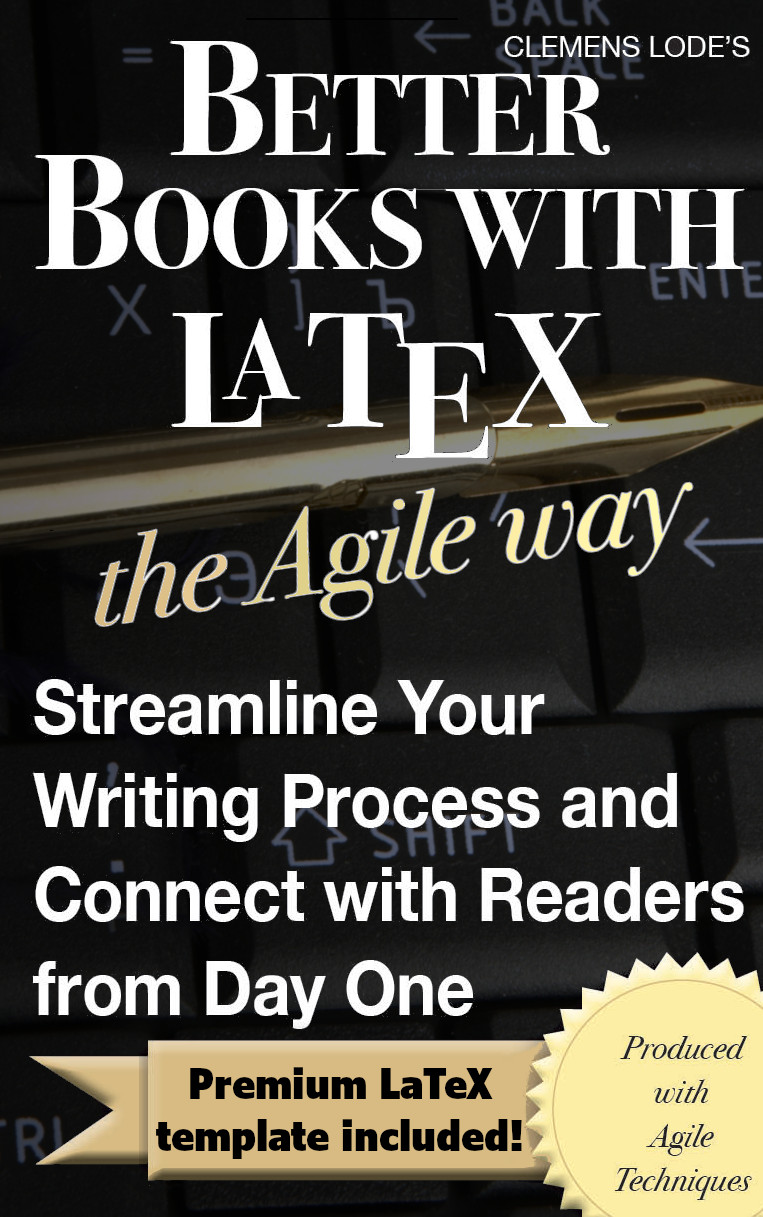
\includegraphics{images/cover.jpg}
	\caption{The cover of this book.}\label{fig:c1_cover}
\end{figure}

In \Cref{fig:c1_cover}, you can see the result of the command. Instead of
graphics, you can also include other TEX files that contain graphics (or
commands to draw graphics, see \Cref{sec:c1_tikzgraphics}).


\section{TikZ Graphics}\label{sec:c1_tikzgraphics}

For graphics, you can use the inbuilt TikZ graphics generator. Due to its
flexibility, I even recommend images you already have for a number of reasons:

\begin{itemize}
    \item TikZ graphics can very easily changed (especially for for example
    translations or making corrections).
    \item TikZ graphics are small and flexible. They can be easily scaled to any
    size and are directly integrated into your project (no time-consuming
    editing in an external graphics program necessary).
    \item TikZ graphics look better. As vector graphics are sent directly to the
    printer, we need not to worry about readability.
\end{itemize}

If you want to create a TikZ graphic, simply create a new TEX file in the
\textit{tex-images} folder and include it with \lstinline[language=Tex]!\input{...}! % chktex 27
(replacing \lstinline[language=Tex]!\includegraphics{}!) where you want to. 

Then, do a ``recompile from scratch'' by clicking on the top right corner of the
preview window (showing Warning or Error) to regenerate the TikZ file. If
``up-to-date and saved'' is shown, delete the \textit{tikz-cache} directory and
recreate it. 

For the format of the file itself, it is a series of commands surrounded by the
\lstinline[language=Tex]!\begin{tikzpicture}...\end{tikzpicture}!%
environment. Discussing all the commands is beyond the scope of this book, so I recommend three options:

\begin{itemize}
    \item Check out the PGF manual at \url{https://www.ctan.org/pkg/pgf}. It is
    more than 1100 pages full with documentation of each command and
    corresponding examples.
    \item Check out the few example TikZ pictures from my two books~\cite{PFH1E, PFH2E} in the \textit{tex-images} directory.
\end{itemize}

\chapter{Replace with Third Chapter Name} \label{c3_thirdchapter:cha}

\begin{figure}
    \centering
    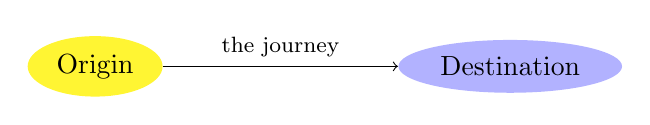
\begin{tikzpicture}
        \node[fill=yellow!80,ellipse] (origin) {Origin};
        \node[fill=blue!30,ellipse] (destination) at (15em,0) {Destination};
        \path (origin) edge[->] node[above,font=\footnotesize] {the journey}
        (destination);
    \end{tikzpicture}
    \caption{TikZ drawings will be output as SVG, which should be rendered by most modern browsers.}
\end{figure}

\begin{figure}
    \centering
    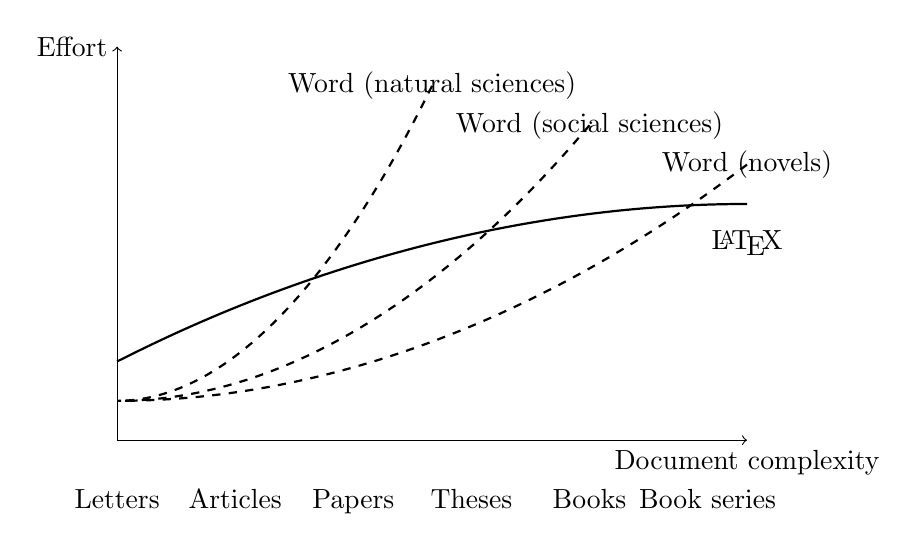
\begin{tikzpicture}

    % horizontal axis
    \draw[->] (0,0) -- (8,0) node[anchor=north] {Document complexity};
    \draw[->] (0,0) -- (0,5) node[anchor=east] {Effort};
    
    % labels
    \draw	(0,-0.5) node[anchor=north] {Letters}
    		(1.5,-0.5) node[anchor=north] {Articles}
    		(3,-0.5) node[anchor=north] {Papers}
    		(4.5,-0.5) node[anchor=north] {Theses}
    		(6,-0.5) node[anchor=north] {Books}
    		(7.5,-0.5) node[anchor=north] {Book series};
    
    \draw (8,3.5) node {Word (novels)};
    \draw (6,4) node {Word (social sciences)};
    \draw (4,4.5) node {Word (natural sciences)};
    \draw (8,2.5) node {\LaTeX{}};
    
    % Psis
    \draw[thick,dashed] (8,3.5) parabola[bend at end] (0,0.5);
    \draw[thick,dashed] (6,4) parabola[bend at end] (0,0.5);
    \draw[thick,dashed] (4,4.5) parabola[bend at end] (0,0.5);
    \draw[thick] (0,1) parabola[bend at end] (8,3);

\end{tikzpicture}
    \caption{Comparing complexity of \textit{Word} and \LaTeX{} depending on the application.}
\end{figure}

\begin{figure}
    \centering
    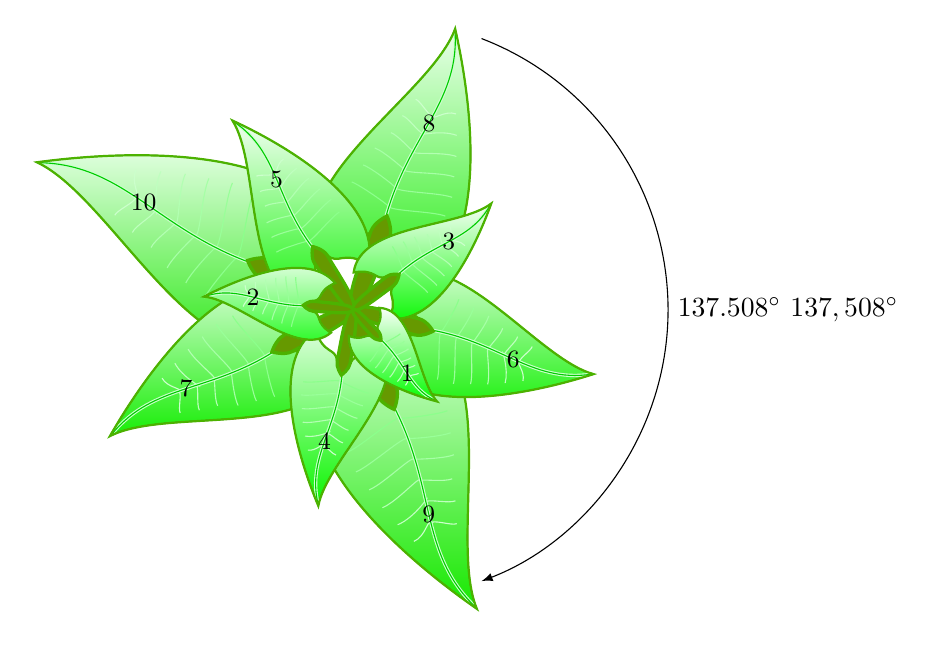
\begin{tikzpicture}
    \foreach \x in {10,...,1}
    {\draw[shade,bottom color=red!\x!green,top color=green!\x,x=0.3 pt,y=0.3 pt,scale={0.4+0.1*\x},rotate=222.5*\x] (0,0) .. 
    controls ( -11,  1) and ( -9, 50) .. (-10,80) ..
    controls ( -16, 60) and (-32, 75) .. (-50,40) .. 
    controls (-110,100) and (-0,230) ..  (  0,300)  node[below] (\x) {} ..
    controls (  45,230) and (110,100) .. ( 50,40) ..
    controls (  32, 75) and ( 16, 60) ..  ( 10,80) ..
    controls (   9, 50) and ( 11,  1) .. (  0,0) 
    -- cycle ;
    
    \draw[thin,green!45,x=0.3 pt,y=0.3 pt,scale={0.4+0.1*\x},rotate=222.5*\x] (-45,120) .. controls (-35,120) and (0,110) .. (-3,110) .. controls (0,105) and (40,120) .. (55,120);
    \draw[thin,green!40,x=0.3 pt,y=0.3 pt,scale={0.4+0.1*\x},rotate=222.5*\x] (-40,140) .. controls (-30,140) and (0,130) .. (-3,130) .. controls (0,125) and (40,140) .. (55,140);
    \draw[thin,green!35,x=0.3 pt,y=0.3 pt,scale={0.4+0.1*\x},rotate=222.5*\x] (-35,160) .. controls (-25,160) and (0,150) .. (0,150) .. controls (0,145) and (35,160) .. (50,160);
    \draw[thin,green!30,x=0.3 pt,y=0.3 pt,scale={0.4+0.1*\x},rotate=222.5*\x] (-25,180) .. controls (-17,180) and (0,170) .. (3,170) .. controls (0,165) and (30,180) .. (45,180);
    \draw[thin,green!25,x=0.3 pt,y=0.3 pt,scale={0.4+0.1*\x},rotate=222.5*\x] (-20,200) .. controls (-13,200) and (0,190) .. (6,190) .. controls (0,185) and (20,200) .. (38,200);
    \draw[thin,green!20,x=0.3 pt,y=0.3 pt,scale={0.4+0.1*\x},rotate=222.5*\x] (-13,220) .. controls (-8,220) and (3,210) .. (8,210) .. controls (10,205) and (18,220) .. (30,220);
    \draw[very thick,green!20,x=0.3 pt,y=0.3 pt,scale={0.4+0.1*\x},rotate=222.5*\x] (0,90) .. controls (-10,180) and (30,230) .. (1,297);
    \draw[thin,black!20!green,x=0.3 pt,y=0.3 pt,scale={0.4+0.1*\x},rotate=222.5*\x] (0,90)  .. controls (-10,180) and (30,230)  .. (1,297) node[midway,black] (num\x) {\small\x};
    \draw[very thick,red!30!green,fill=red!40!green,x=0.3 pt,y=0.3 pt,scale={0.4+0.1*\x},rotate=222.5*\x] 
    (0,0) .. 
    controls ( -11,  1) and ( -9, 50) ..
    (-10,80) .. 
    controls (-10,90) and (0,100) .. (0,100) ..
    controls (0,100) and (10,90) .. (10,80)..
    controls (   9, 50) and ( 11,  1) .. (  0,0) 
    -- cycle;
    \draw[thick,red!30!green,x=0.3 pt,y=0.3 pt,scale={0.4+0.1*\x},rotate=222.5*\x] (0,0) .. 
    controls ( -11,  1) and ( -9, 50) .. (-10,80) ..
    controls ( -16, 60) and (-32, 75) .. (-50,40) .. 
    controls (-110,100) and (-0,230) ..  (  0,300) ..
    controls (  45,230) and (110,100) .. ( 50,40) ..
    controls (  32, 75) and ( 16, 60) ..  ( 10,80) ..
    controls (   9, 50) and ( 11,  1) .. (  0,0) 
    -- cycle ;
    }
    \draw[->,>=latex,x=0.3 pt,y=0.3 pt,black] ([xshift=6pt] 8.east) arc (69:-69:350) node[midway,right] {$137.508^\circ$ $137,508^\circ$};
\end{tikzpicture}


    \caption{Example of a drawing made in TikZ.}
\end{figure}



\chapter{Fault Attacks} \label{c9_ninthchapter:cha}

\begin{centering}
	\section*{Topics}
		\begin{enumerate}
			\begin{centering}
				\item Introduction to Fault Attacks
				\item Fault Attack on RSA-CRT
				\item DRAM and Rowhammer
				\item Flip-Feng-Shui: Rowhammer attack on RSA \\
			\end{centering}
		\end{enumerate}
\end{centering}
\newpage
\section*{Introduction to Fault Attacks}
Up until now in the course we learned about \emph{passive} attacks -- i.e. attacks which measure \emph{leakage} such as timing information and power traces. The advantage of these attacks is that they allow an attacker to acquire information in the process of an ongoing computation e.g. an AES key \emph{before} it was fully mixed with the input -- this fact can help the attacker extract secrets.

In fault attacks we will become \emph{active} in the sense that we will give the device-under-test (DUT) additional inputs such as heat or radiation.

One problem with Fault attacks: they use the strongest attack model, meaning -- we assume most power on the attacker's part.

\section{Active Attacks}
\paragraph{Definition:}
\begin{quote}
	\textit{"A fault attack is an active attack that allows extraction of secret information from cryptographic devices by breaking those devices."}
\end{quote}

In fault attacks we are being \emph{active} -- we give additional inputs beside the main input such as:
\begin{enumerate}
	\item Fuzzing (garbage or bad input)
	\item Radiation
	\item Heat
	\item Vibration
	\item Power spikes etc.
\end{enumerate}

This way, we receive other (usually erroneous) outputs which might give us additional information about the computation and/or the secret. This process is described in \cref{fig:fault_attacks_schematic}.

\begin{figure}[!ht]
	\centering
	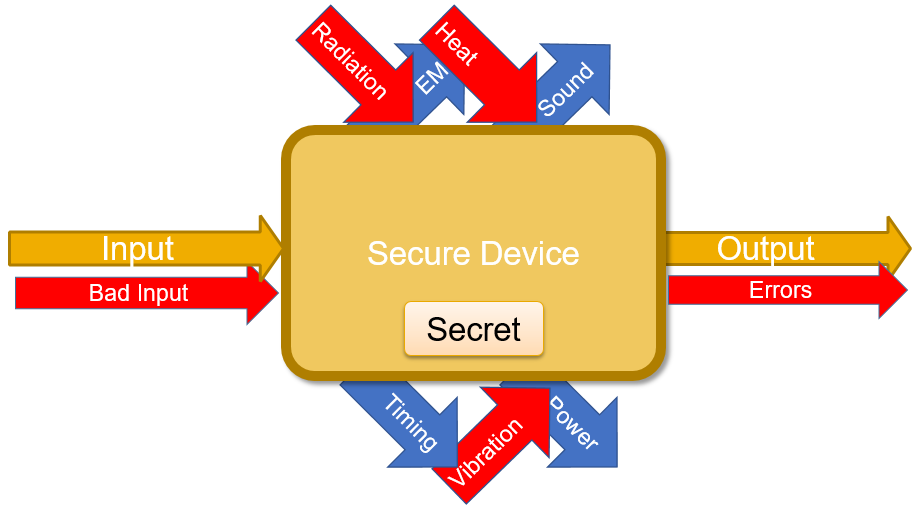
\includegraphics[width=0.7\linewidth]{images/ch9/fault_attacks_schematic.png}
	\caption{A schematic diagram of fault attacks and leakage types.}
	\label{fig:fault_attacks_schematic}
\end{figure}

Like with passive attacks, some of those outputs can be acquired at different stages of the computation process.

Many fault attacks are inspired by studies in the field of \emph{reliability}: a study in reliability will research a device's physical boundaries e.g. the maximum or minimum temperature under which it performs reliably. Other examples of reliability studies are aimed at improving device performance under extreme conditions such as:
\begin{itemize}
	\item Space and X-Rays
	\item Dense CPU Layouts
	\item Data Center Recovery (ECC-RAM)
\end{itemize}

A security researcher implementing fault attacks will, on the other hand,  purposefully subject the DUT to extreme conditions in order to inject errors in the device's functionality to achieve their goal. In that sense, a reliability study of a given device can lay the ground-work for the fault attacks to come.

\begin{quote}
	\textit{"In the reliability community things happen by mistake. In the security community -- things happen on purpose."}
\end{quote}

\subsubsection*{Breaking a device-under-test}
How can \emph{breaking} a device help an attacker?

\begin{enumerate}
	\item BORE -- \textit{"Break Once, Run Everywhere"}: Some device families share a single secret among all instances.
	\item Repairable Devices: Temporary breakage is fine. Sometimes restarting the device is enough to "repair" the damage.
	\item Partial breakage: Sometimes it's convenient to break \emph{part} of a device, for example -- destroy the subsystem responsible for DRM verification.
\end{enumerate}

\section{Fault Attack Taxonomy}
The tree ways we can examine a Fault Attack in order to understand it are:
\begin{enumerate}
	\item Method - \emph{"How to inject?"}
	\item Properties - \emph{"What fault to create?"}
	\item Target - \emph{"Which part to break?"}
\end{enumerate}

\subsection{Fault Methods}

\subsubsection{Power Supply Attacks}
What happens if the device is underpowered?
As we have previously seen, power in electronic devices is used to drive the CMOS transistors. If the device is slightly underpowered it might fail to switch some of the transistors and thus produce false calculations, and with even less power it might  struggle with getting into operational state (boot loop) or even transition to an entirely faulty state.
Another attack method involving the power supply is injecting power spikes (to a similar effect).

Some parts of a device are typically more sensitive to the power supply than others, and thus under- or over-powering the device will de-stabilize it and inject faults.

The obvious scenario for such an attack is when the DUT belongs to or is being controlled by the attacker -- for example if they're examining their own set-top box etc. In that case, the attacker can supply the device with as much/little power as they wish.

Another example of such attack scenarios is in the field of RFID readers -- the device powering an RFID chip is the reader, so a \emph{malicious} RFID reader can over/under-power the chip to achieve various faulty results.

\subsubsection{Clock/Timing Attacks}
The clock is typically a bus shared by many of the system's components which synchronizes the propagation of calculations through the system -- i.e. at the beginning all inputs are ready, and when there is a rising edge on the clock bus they start propagating throughout the various computational components. When all computations are finished they all wait for the next rising edge on the clock bus in order to proceed to the next stage.
In a clock glitching attack the attacker would inject a rising edge on the clock bus at an arbitrary time. This way only \emph{some} of the computations will have finished by that time while others are still being processed, and thus the device will be in a faulty (unstable) state.

A notable example is the attack on Mifare Classic RFID chips we talked about in the beginning of the course \cite{nohl2008} -- the RNG in the chip is only dependent on the time between powering up the RFID tag and challenging it. An RFID reader operated by the attacker can control both parameters, thus making the generated challenges deterministic.

\subsubsection{Temperature attacks}
This attack method relies on the physical property of electrons (current). Electrons  "jump", and the higher the temperature -- they will jump more frequently and to longer distances.
If a device gets \emph{too hot} -- enough electrons can "jump" e.g. over the insulation layer in a transistor to flip it from logical 1 to 0. This results in a fault.

Because of the ubiquity of devices failures due to temperature, nowadays temperature sensors are integrated into most devices, so when it overheats -- the device will shut down.

An attacker can bypass the temperature sensor by disconnecting it. Another method would be to quickly alternate the temperature of the device from extremely high to extremely low, so that \emph{on average} the temperature is reasonable, but it will still experience faults during the extreme phases of the cycles.

In an interesting research paper \cite{appel} a type-confusion attack on the Java virtual-machine was demonstrated: at first, the entire memory was filled with small arrays (say of size one). The Java VM is type-safe, so it is normally impossible to access one of the memory regions using a pointer to a different region. To inject a type-confusion fault the researchers used a 50W light bulb to heat the memory chip of the device enough to flip some of the bits (for illustration see \cref{fig:memory_lightbulb}). As a result, a small portion of the data-structures describing the arrays in memory now held wrong values (e.g. changed their value from $size=1$ to $size=20$). At this point, some affected data-structure \emph{contains} a header of a different data-structure, to which the attackers now have read and write access. Changing the header of the second data structure to an arbitrary value gave the attackers access to the entirety of the device's memory.
\begin{figure}[!ht]
	\centering
	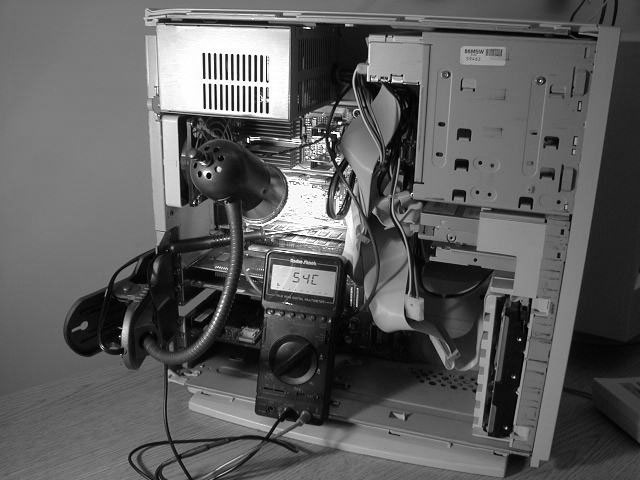
\includegraphics[width=0.7\linewidth]{images/ch9/bulb.png}
	\caption{A light bulb flipping memory bits filled with safe Java structures.}
	\label{fig:memory_lightbulb}
\end{figure}

\subsubsection{Optical, Electromagnetic}
When a laser hits a transistor it changes the energy level of the silicon inside, and sometimes it can change the transistor's state. Notably different wavelengths are absorbed by different materials, so in a typical silicon chip different lasers will hit different layers of the device etc. Magnetic/Electromagnetic radiation and pulses have similar effects.

The underlying principal of those attacks is that the attacker forcefully injects charge (energy) into the device. Once it's stored inside it will have to dissipate one way or another, so as a result it injects a random faulty state into the device.

\subsubsection{Reading from RAM}
All of the attacks described above require very high engagement with the DUT -- in order for the attacker to control the power/clock sources, for example, they sometimes would need to drill, cut or otherwise tamper with the device. Shining a laser on a device requires at the very least having it at a visible distance.

The final attack method involves only \emph{reading} from memory, and thus is very practical and requires very little physical engagement. This attack method is called \emph{Rowhammer} and is discussed later in the lecture.


\subsection{Fault Properties}
In this section we discuss:
\begin{enumerate}
	\item How controllable is the fault's location/size? Precise? Loose? None?
	\item How controllable is the fault timing?
	% Can we have the fault occur when something exciting is happening?
	% Heat is the LEAST controllable -- it's a gradual and stochastic process. Freaking Lasers -- very controllable.
	\item What's the fault's duration? Transient? Permanent? Destructive?
\end{enumerate}


\subsubsection*{Destructive fault attacks on cryptographic devices}
What can be done with fault attacks to symmetric ciphers?
\paragraph{Easy example:} Imagine that we have a pile of cipher devices with a 64bit key length, which work the following way: we can give the device a key and it tells us whether it's the right key.

What if we have a DESTRUCTIVE fault attack that resets the top 32bits of a device's key? We can brute force the key in $2\cdot2^{31}$ instead of $2^{63}$ (on average):

First we inject the fault into one of the devices and brute-force the lower 32 bits of the key ($O(2^{31})$), then we pick another device from the pile and brute-force only the higher 32 bits (another $O(2^{31})$).

\paragraph{A less trivial example:} We have a public-key device which we can ZAP and one bit of the key flips to zero.

We can save all of the plaintexts-cipher pairs until we reach the one matching an all zero key -- which we can pre-calculate. This gives us the Hamming weight of the key.
Now we go back one plaintext-cipher pair -- we know that pair's key's Hamming weight to be exactly one -- meaning we need to brute-force only $N$ keys ($N$ is the key bit-length). Now we have the position of a single bit of the key.

If we iterate all the way backwards to the original plaintext-cipher pair, we can acquire the key in $O(N^2)$ time!

\subsection{Fault Target}
What could be targeted by a fault attack?
\begin{enumerate}
	\item Input parameters (fuzzing, clock glitching)
	\item Storage (volatile/non-volatile)
	\begin{enumerate}
		\item HDD - Destructive (persists after reset)
		\item RAM - Permanent
		\item Cache - Transient
	\end{enumerate}
	% If we fault the disk/flash? It's a destructive fault! If we fault the RAM, the fault is permanent (not destructive). In cache? Transient fault!
	% What other storage is there? Instruction cache.
	\item Data processing: inject a fault mid-computation and the device gives a different answer.
	\item Instruction Processing/Control Flow: inject a fault in the IP register and change the instruction flow.
	\begin{enumerate}
		\item ARM32 instructions are very densely packed, thus there is a very high probability of hitting a valid instruction after flipping a single bit. \texttt{jnz} and \texttt{jmp} are only one bit apart.
		\item Change for loop condition to dump RAM contents including source code.
	\end{enumerate}
\end{enumerate}

\paragraph{Two examples of Fault Attacks targeting Control Flow:}
\begin{enumerate}
	\item The CHDK hacking community, used to dump the firmwares of Canon cameras via blinking one of their LEDs \cite{chdk, bib:canon}.

	\item "The Unlooper": Back in the 90's pay-tv devices started cryptographically signing the content, and if the cryptographic checksum did not check out -- the device would enter an endless loop. The hacking community invented "unloopers" -- a gadget that would inject a power spike and fault the IP register, so that the pay-tv device would jump to some other section of the code, from which point it would function normally.
\end{enumerate}

\section{Fault attack on RSA-CRT}

\subsection{RSA decryption}
\[
	N = p\cdot q
\]
\[
	M = C^d (mod\ n) = M^{ed} (mod\ n) = M^1 (mod\ n)
\]

RSA decryption is hard!

Let's speed it up using CRT (the Chinese Remainder Theorem):
Multiplication operations are $O(|n|^2)$. If we can do operations $(mod\ p)$ and then $(mod\ q)$ instead of $(mod\ n)$, we will reduce computation time by half.

\paragraph{Explanation:}

The bit-lengths of $p$ and $q$ are each half that of $n$
\[|p|=|q|=\frac{1}{2}|n|\]
The computational complexity of multiplying by a number of length $x$ is (roughly) $O(x^2)$. Thus:
\[
O(|p|^2) = O(|q|^2) = \frac{1}{4}O(|n|^2) \Rightarrow (O(|p|^2) + O(|q|^2)) = \frac{1}{2}O(|n|^2)
\]

So if we could multiply by $p$ and $q$ instead of by $n$, we would cut \emph{each} multiplication operation's time complexity in half!

\subsubsection{Chinese Remainder Theorem}
\begin{figure}[!ht]
	\centering
	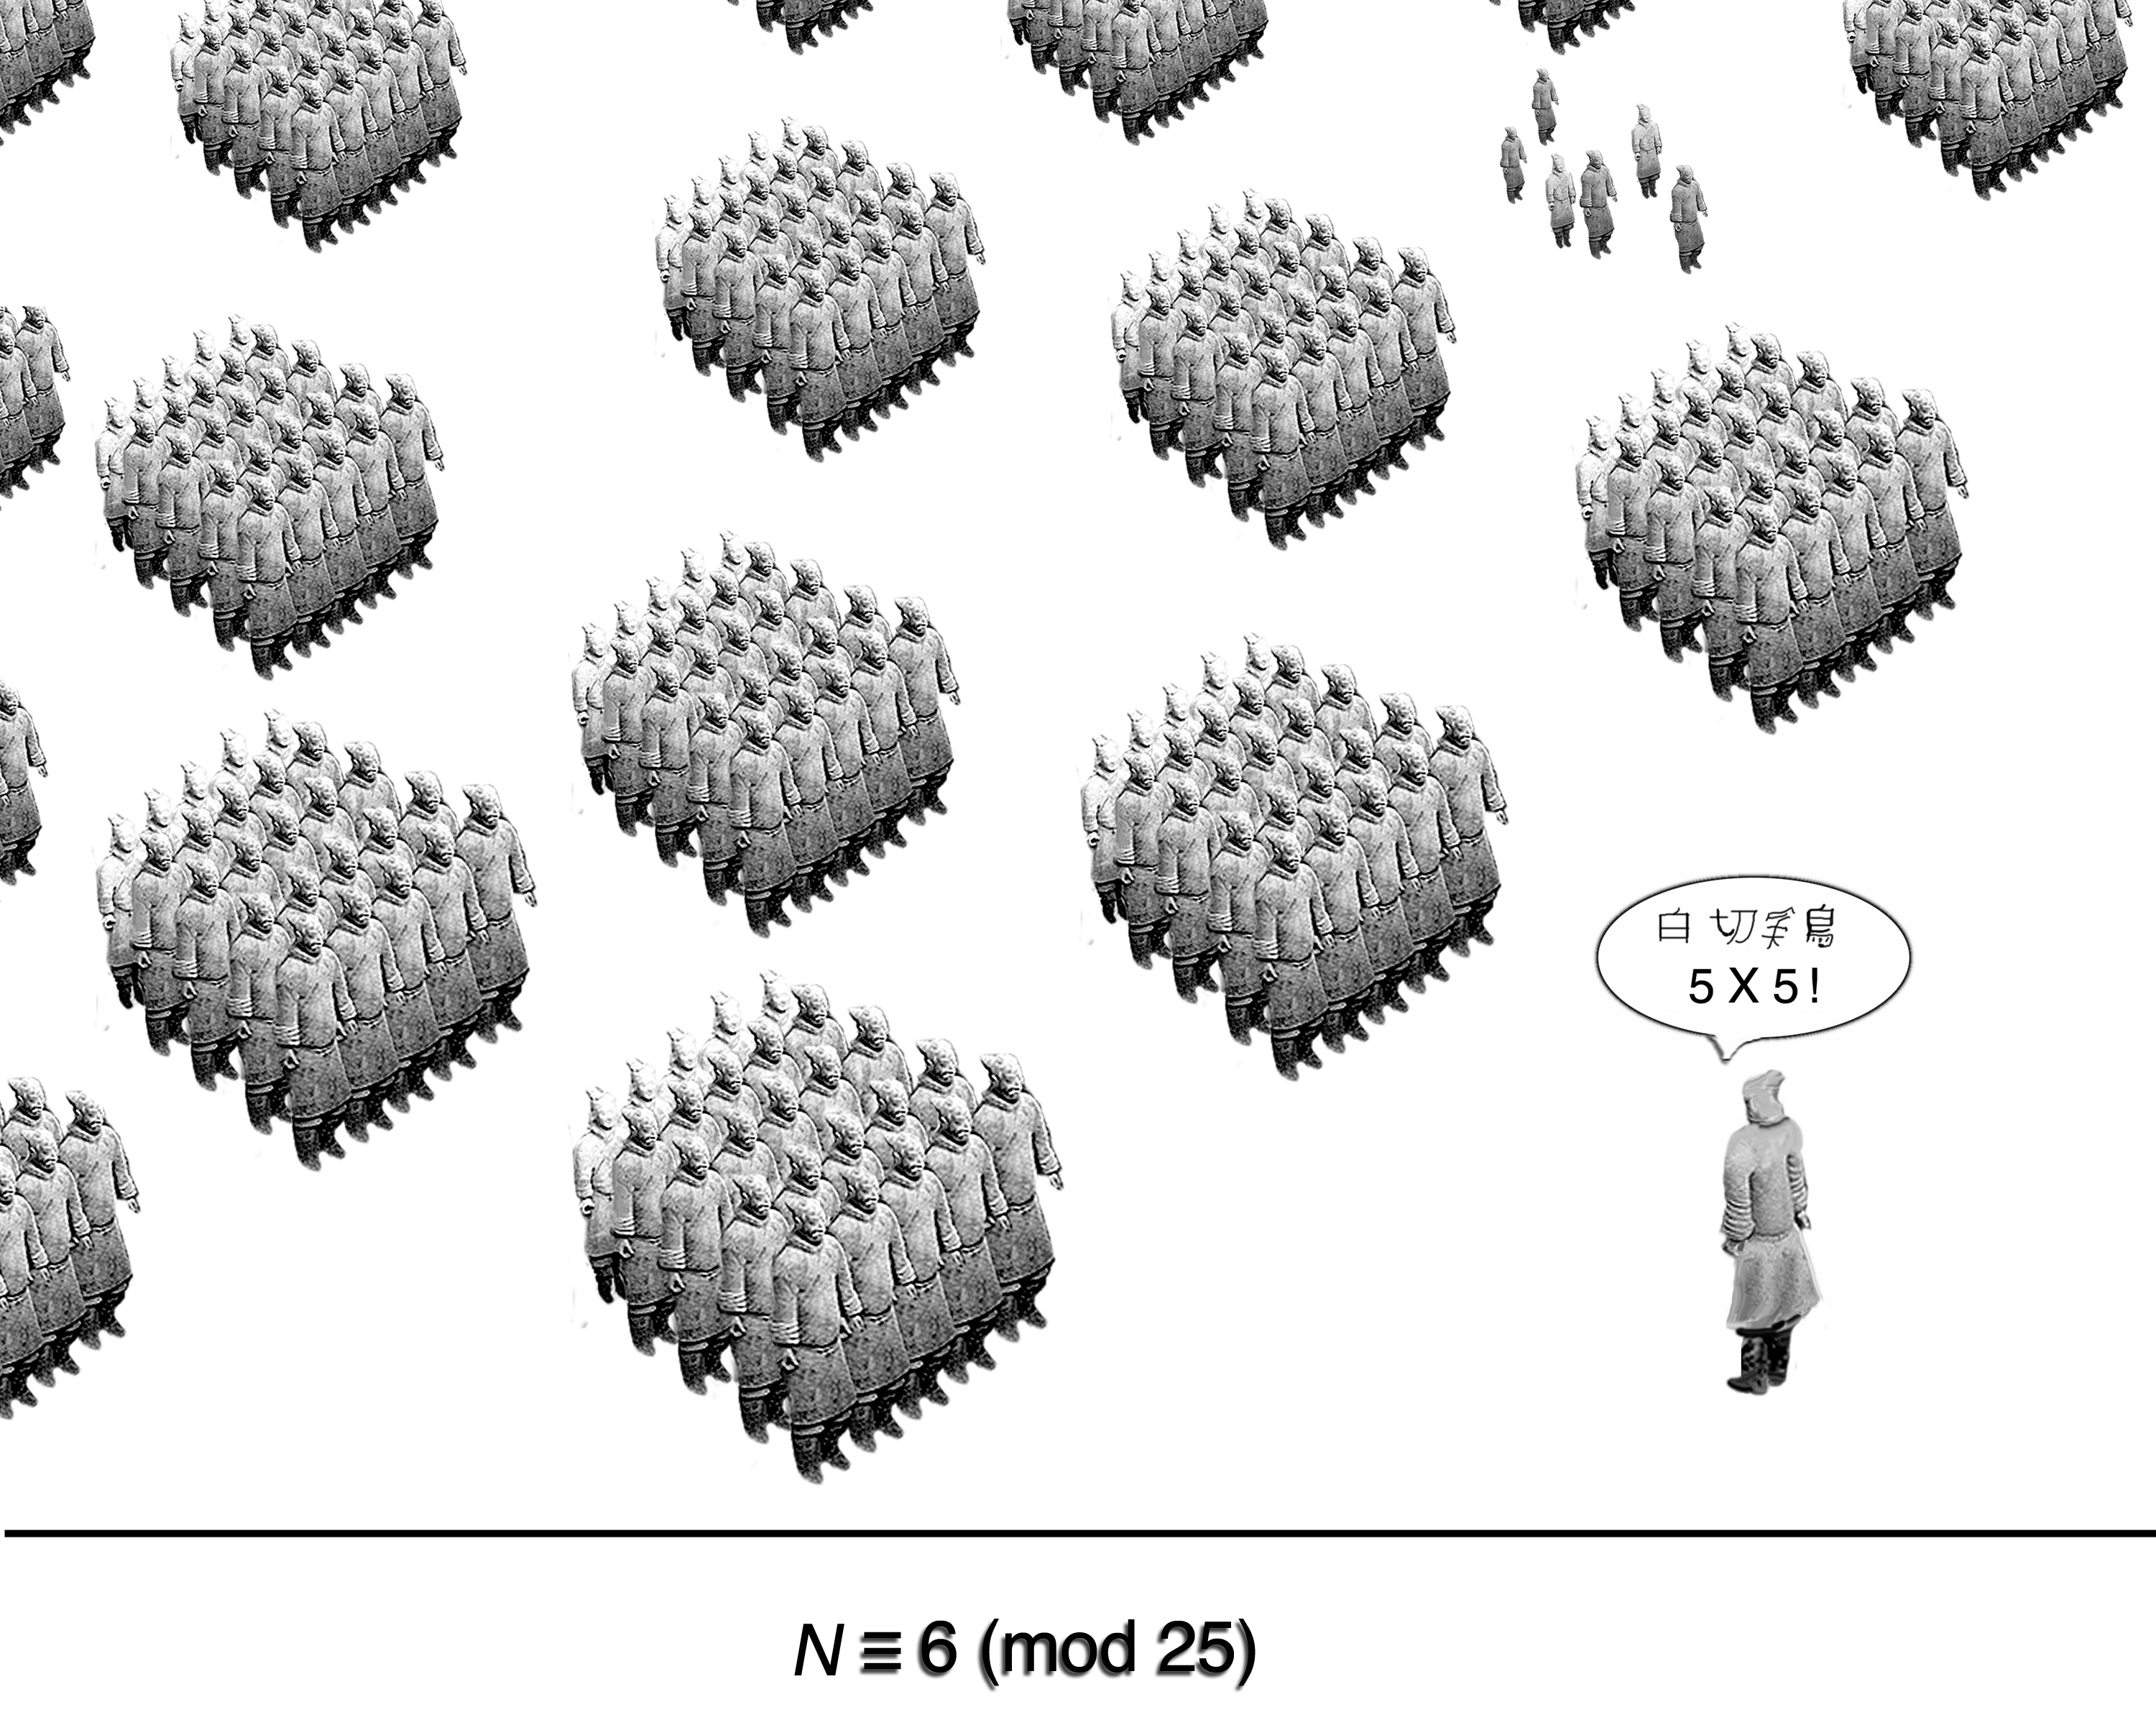
\includegraphics[width=0.5\linewidth]{images/ch9/soldiers.jpeg}
	\caption{Chinese Remainder Theorem (Source: \url{https://russinoff.com/papers/crt.html})}
	\label{fig:chinese_remainder}
\end{figure}
The idea is that if we know both $x (mod\ p)$ and $x (mod\ q)$ then we can easily calculate $x (mod\ n)$.

So, given a message $M$ calculate $M_p$ and $M_q$:
\[M_p = C^d (mod\ n)(mod\ p) = C^d (mod\ p)\]
\[M_q = C^d (mod\ n)(mod\ q) = C^d (mod\ q)\]

To combine the values, we do:
\[
	M^* = CRT(M_p, M_q) = M_p \cdot q \cdot (q^{-1} mod\ p) + M_q \cdot p \cdot (p^{-1} mod\ q)
\]

It is easily provable that \(M^*(mod\ p)=M_q\) and \(M^*(mod\ q)=M_p\), so by the Chinese Remainder Theorem, this value \emph{must} be equal to $M$.

\subsubsection{The Boneh, DeMillo \& Lipton Fault Attack on RSA-CRT \cite{boneh}}

The attacker has a decryption box (known plaintext scenario) with public key $n$ and would like to recover $d$ (the private key). Additionally, the attacker knows that the decryption box is decrypting using CRT. Finally, let us assume that the attacker can inject a fault (any fault) in the decryption process.

The attacker first gets \(M = M_p*q*(q^{-1} mod\ p) + M_q*p*(p^{-1} mod\ q)\)
through the regular decryption process.

Then, the attacker primes the device to re-calculate the message from the same cipher, this time injecting a \emph{fault} during the calculation of $M_p$, resulting in the device erroneously producing $M'_p$ instead:
\[M'_p \neq C^d (mod\ p)\]
The device will then proceed to combine $M'_p$ with the correct result of $M_q$, resulting in:
\[M' =  M'_p \cdot q \cdot (q^{-1} mod\ p) + M_q \cdot p \cdot (p^{-1} mod\ q)\]

Now the attacker can calculate the value of $M - M'$:
\[
	 (M_p \cdot q \cdot (q^{-1} mod\ p) + M_q \cdot p \cdot (p^{-1} mod\ q)) - (M'_p \cdot q \cdot (q^{-1} mod\ p) + M_q \cdot p \cdot (p^{-1} mod\ q)) =
\]
\[
	(M_p - M'_p) \cdot q \cdot (q^{-1} mod\ p))
\]

Finally, calculating the $gcd$ of $n$ and $M - M'$ yields:
\[
	\gcd(n, M - M') = \gcd(p \cdot q, (M_p - M'_p) \cdot q \cdot (q^{-1} mod\ p)) = q
\]

\paragraph{Why does this work?} The greatest common divisor of $n$ and anything can be only $p$, $q$, $n$ or $1$. On the other hand, $M_p$ and $M'_p$ can never be multiples of $p$, otherwise both would equal 0. So, by that reasoning, $\gcd(p \cdot q, (M_p - M'_p) \cdot q \cdot (q^{-1} mod\ p))$ \underline{must} equal $q$, and thus we have cracked the cipher using a single fault attack.

A later paper co-written by Arjen Lenstra \cite{lenstra} further improved upon this attack to not require knowledge of $M$.

\paragraph{BML in practice:} A paper \cite{schmidt} showed how ZAPPING a device with an electric spark from a lighter during computation can achieve the described effect.

\section{Rowhammer}
In the final section, we will describe the Rowhammer attack.
\subsection{Rowhammer attack taxonomy}
	\begin{itemize}
		\item Target: DRAM on modern computers
		\item Properties: Permanent, controlled location
		\item Method: Memory accesses
	\end{itemize}

\begin{figure}[!ht]
	\centering
	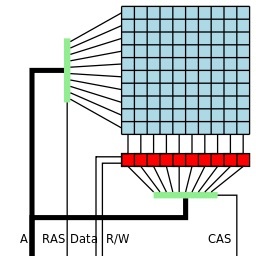
\includegraphics[width=0.5\linewidth]{images/ch9/DRAM.jpg}
	\caption{High Level Illustration of DRAM Organization (Source: Wikipedia:Row Hammer)}
	\label{fig:dram_svg}
\end{figure}

\subsection{Double-sided Rowhammer}
DRAM is the most common type of volatile memory. It is slow, dense and cheap relatively to SRAM. Every bit of RAM is stored in a single capacitor.

The attack \cite{rowhammer} utilizes the physical structure of RAM chips in order to induce faults: Due to parasitic leakage in DRAM capacitors, if enough consecutive reads are performed on the immediately adjacent rows eventually a bit will flip in the target row.

\subsubsection{The challenge of CPU caching}
The CPU cache prevents the same memory address to be read consecutively from main memory, for performance reasons.
To circumvent this limitation, several techniques can be employed:
\begin{enumerate}
	\item Intel CPUs provide non-temporal read/write opcodes -- special instructions that read from memory and don't get cached.
	\item The special \texttt{clflush} instruction can be used to explicitly flush the cache after each read operation (privileged operation).
	\item Finally, cache-population algorithms had been extensively studied and reverse-engineered, so it is possible to arrange for \emph{arbitrary} cache misses.
\end{enumerate}

\subsection{Countermeasures}
\paragraph{Refresh-rate increase:} In order to overcome parasitic leakage, DRAM chips already have a mechanism in place to read and then re-write the values stored in each row periodically. One method of overcoming Rowhammer could be to significantly increase the refresh-rate of the chip. This obviously results in both performance degradation and increased power consumption.

\paragraph{ECC-RAM:} High-end DRAM chips (typically meant for data center environments) contain error-correction coding (ECC) logic which can typically \emph{correct} one erroneous bit and \emph{detect} two (at which point it will crash the program/system). Those chips are immune to the basic form of Rowhammer described above, but as discussed later, are not bullet-proof.

\subsection{Rowhammer variations}
\subsubsection{Flip Feng-Shui}
\paragraph{Page de-duplication:} On modern systems, typically much memory is shared among many processes running on the system. This is even more true of virtualized environments where the guest and the host, for example, could run the same OS. A common optimization is for the system to detect and de-duplicate pages containing the same data, thus freeing up memory.
\paragraph{Rowhammer + page de-duplication:}
In a paper \cite{ffs} researchers from VUA demonstrated how they can utilize page-deduplication in a virtualized environment to weaken cryptographic keys, resulting in unauthorized access via OpenSSH, and breach of trust via forging GPG signatures. The attack relies on the fact that the the attacker can \emph{read} a de-duplicated page as much as they want. The attacker has to wait (or arrange) for a page containing sensitive information to be de-duped, then hammer on it until a bit in the key flips, making it much easier to factor.
\begin{figure}[!ht]
	\centering
	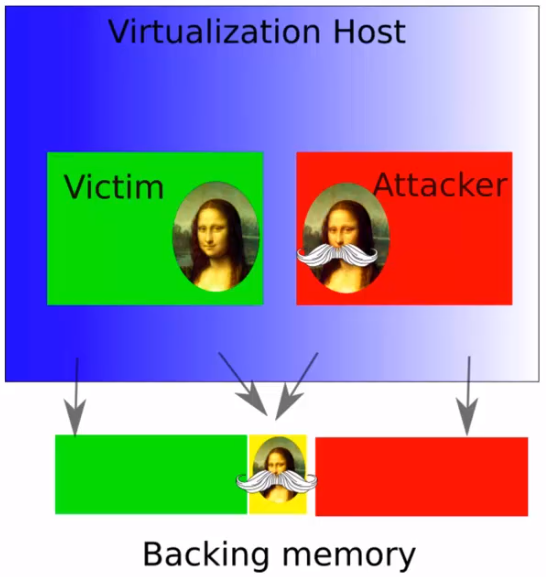
\includegraphics[width=0.5\linewidth]{images/ch9/flip_feng_shui.PNG}
	\caption{The attacker maps the same page as the victim, then utilizes rowhammer to change the victim's memory without causing page duplication.}
	\label{fig:flip_feng_shui}
\end{figure}

\subsubsection{ECCPloit}
In another paper \cite{eccploit} researchers from VUA showed how they can use Rowhammer to quickly flip \emph{enough} (typically three) bits on an ECC-RAM chip that error correction will not be able to detect it, thus defeating the ECC mitigation. The attack relies on the fact that error-correction takes time to compute, and this gives the attacker a window of opportunity.


\clearpage
\bibliographystyle{unsrt}
\bibliography{bibliography/english}

\end{document}